\chapter{Evaluation}
\label{ch:Evaluation}

In this chapter, we will look at the results of the different models. 
We first evaluate which features are most important for the models using 
permutation feature importance, then we will look at the pinball scores from 
that are used in the competition. Finally, we will look at how the models performed 
considering another scoring function, the Energy score.

\section{Feature importance}

One way to determine the importance of a feature for a model is called 
permutation feature importance. Here, the model is trained like usual but for the prediction 
step, we don't use the normal test data, but a modified dataset where one feature is 
shuffled. Like that, the model cannot use the information of this feature properly 
and will most likely perform worse. The performance on the shuffled dataset is 
then divided by the performance on the regular test set. A value close to \(1\) 
indicates that the feature is not that important because the model doesn't perform 
much worse than before. The higher the quotient, the more important the feature is for the model.
Since our time series heavily depends of the time of day, it makes sense 
not to shuffle the whole feature but only the equivalence classes of each hour, 
i.e. the values at \(1\) AM are shuffled, the values at \(2\) AM are shuffled, etc.

Table \ref{table:feature-importance} and Figure \ref{fig:feature-importance} 
show the results of the permutation feature importance calculation.

\begin{table}[h!]%
    \rowcolors{2}{white}{gray!25}
    \centering
    \footnotesize
    \begin{tabular}{lllllll}
    \toprule \noalign{\smallskip}
    \tableheads Model & \tableheads SSRD & \tableheads STRD & \tableheads TSR & \tableheads TP & \tableheads TCC & \tableheads Previous points \\ 
    \midrule
    QRF     & \(1.3365\) & \(1.0214\) & \(1.0199\) & \(1.0020\) & \(1.0025\) & -- \\
    NNQF    & \(1.2202\) & \(1.0052\) & \(1.0856\) & \(1.0032\) & \(1.0405\) & -- \\
    SQF-RNN & \(1.0268\) & \(1.0208\) & \(1.0516\) & \(1.0124\) & \(1.2059\) & \(1.0918\) \\
    \bottomrule
    \end{tabular}

    \caption[Feature importance]{Feature importance. 
    The table shows the permutation feature importance quotients. 
    The permutation feature importance quotient is 
    the performance of the model with shuffled feature 
    divided by the performance of the model without shuffled features. 
    A higher value indicates a more important feature.}
    \label{table:feature-importance}    
\end{table}

\begin{figure}[h!]
    \begin{tikzpicture}
    \begin{axis}[
        width  = \textwidth,
        height = 0.3\textheight,
        major x tick style = transparent,
        ybar,
        bar width=10pt,
        ymajorgrids = true,
        ylabel = {Feature importance},
        xtick = {1,2,3,4,5,6},
        xticklabel style={align=center},
        xticklabels = {Surface\\solar\\rad down, Surface\\thermal\\rad down, Top net\\solar rad, Total\\precipitation, Total\\cloud cover, Previous\\points},
        scaled y ticks = false,
    ]
        \addplot
            coordinates {(1, 1.3365) (2, 1.0214) (3, 1.0199) (4, 1.0020) (5, 1.0025)};
        \addplot
            coordinates {(1, 1.2202) (2, 1.0052) (3, 1.0856) (4, 1.0032) (5, 1.0405)};
        \addplot
            coordinates {(1, 1.0268) (2, 1.0208) (3, 1.0516) (4, 1.0124) (5, 1.2059) (6, 1.0918)};

        \legend{QRF, NNQF, SQF-RNN}
    \end{axis}
\end{tikzpicture}
    \caption[Feature importance]{Feature importance. 
    The table shows the permutation feature importance quotients. 
    The permutation feature importance quotient is 
    the performance of the model with shuffled feature 
    divided by the performance of the model without shuffled features. 
    A higher value indicates a more important feature.}
    \label{fig:feature-importance}
\end{figure}
\todo{same caption as before?}